\chapter{ANÁLISES}
\label{chap:analyze}

Foram realizados 3 testes consecutivos em 4 máquinas diferentes, sendo elas:

\begin{table}[H]
    \caption{Configurações da máquinas onde reproduziram-se os testes.}
    \label{tab:config_timon}
    \begin{tabular}{|l|l|l|l|}
    \hline
    \multicolumn{1}{|c|}{Máquina 1} & \multicolumn{1}{c|}{Máquina 2} & \multicolumn{1}{c|}{Máquina 3} & \multicolumn{1}{c|}{Máquina 4} \\ \hline
    \begin{tabular}[c]{@{}l@{}}Nome: Jéssica\\ CPU: i7 9750H\\ GPU: GTX 1660 Ti\\ RAM: 8GB DDR4\\ Real time factor: 0,6\end{tabular} & \begin{tabular}[c]{@{}l@{}}Nome: Leonardo\\ CPU: FX 6300\\ GPU: GTX 750 Ti\\ RAM: 4GB DDR3\\ Real time factor: 0,37\end{tabular} & \begin{tabular}[c]{@{}l@{}}Nome: Miguel\\ CPU: i7 4790\\ GPU: GT 730\\ RAM: 16GB DDR3\\ Real time factor: 0,45\end{tabular} & \begin{tabular}[c]{@{}l@{}}Nome: Vinicius\\ CPU: i7 8550U\\ GPU: GeF. MX150\\ RAM: 8GB DDR3\\ Real time factor: 0,3\end{tabular} \\ \hline
    \end{tabular}
    \legend{Fonte: Autoria própria.}
    \end{table}

    O objetivo do teste foi registrar o tempo que cada robô Darwin-OP levava para realizar o seu percurso na corrida de revezamento.


    % Please add the following required packages to your document preamble:
% \usepackage[table,xcdraw]{xcolor}
% If you use beamer only pass "xcolor=table" option, i.e. \documentclass[xcolor=table]{beamer}
% Please add the following required packages to your document preamble:
% \usepackage[table,xcdraw]{xcolor}
% If you use beamer only pass "xcolor=table" option, i.e. \documentclass[xcolor=table]{beamer}
\begin{table}[H]
    \caption{Dados coletados dos testes realizados.}
    \label{tab:dados_timon}
    \begin{tabular}{|c|c|c|c|lc|c|c|c|}
    \cline{1-4} \cline{7-9}
    \cellcolor[HTML]{9B9B9B}{\color[HTML]{000000} \textbf{Máquina}} & \cellcolor[HTML]{9B9B9B}{\color[HTML]{000000} \textbf{Teste}} & \cellcolor[HTML]{9B9B9B}{\color[HTML]{000000} \textbf{Robô}} & \cellcolor[HTML]{9B9B9B}{\color[HTML]{000000} \textbf{Tempo (s)}} & {\color[HTML]{000000} } & \multicolumn{1}{l|}{\cellcolor[HTML]{9B9B9B}{\color[HTML]{000000} \textbf{Máquina}}} & \cellcolor[HTML]{9B9B9B}{\color[HTML]{000000} \textbf{Teste}} & \cellcolor[HTML]{9B9B9B}{\color[HTML]{000000} \textbf{Robô}} & \cellcolor[HTML]{9B9B9B}{\color[HTML]{000000} \textbf{Tempo (s)}} \\ \cline{1-4} \cline{6-9} 
    1 & 1 & 1 & 62,210 & \multicolumn{1}{l|}{} & 3 & 1 & 1 & 66,859 \\ \cline{1-4} \cline{6-9} 
    \cellcolor[HTML]{C0C0C0}1 & \cellcolor[HTML]{C0C0C0}1 & \cellcolor[HTML]{C0C0C0}2 & \cellcolor[HTML]{C0C0C0}67,055 & \multicolumn{1}{l|}{} & \cellcolor[HTML]{C0C0C0}3 & \cellcolor[HTML]{C0C0C0}1 & \cellcolor[HTML]{C0C0C0}2 & \cellcolor[HTML]{C0C0C0}67,673 \\ \cline{1-4} \cline{6-9} 
    1 & 1 & 3 & 65,496 & \multicolumn{1}{l|}{} & 3 & 1 & 3 & 66,132 \\ \cline{1-4} \cline{6-9} 
    \cellcolor[HTML]{C0C0C0}1 & \cellcolor[HTML]{C0C0C0}1 & \cellcolor[HTML]{C0C0C0}4 & \cellcolor[HTML]{C0C0C0}68,529 & \multicolumn{1}{l|}{} & \cellcolor[HTML]{C0C0C0}3 & \cellcolor[HTML]{C0C0C0}1 & \cellcolor[HTML]{C0C0C0}4 & \cellcolor[HTML]{C0C0C0}68,500 \\ \cline{1-4} \cline{6-9} 
    1 & 2 & 1 & 64,352 & \multicolumn{1}{l|}{} & 3 & 2 & 1 & 63,283 \\ \cline{1-4} \cline{6-9} 
    \cellcolor[HTML]{C0C0C0}1 & \cellcolor[HTML]{C0C0C0}2 & \cellcolor[HTML]{C0C0C0}2 & \cellcolor[HTML]{C0C0C0}67,405 & \multicolumn{1}{l|}{} & \cellcolor[HTML]{C0C0C0}3 & \cellcolor[HTML]{C0C0C0}2 & \cellcolor[HTML]{C0C0C0}2 & \cellcolor[HTML]{C0C0C0}68,312 \\ \cline{1-4} \cline{6-9} 
    1 & 2 & 3 & 68,063 & \multicolumn{1}{l|}{} & 3 & 2 & 3 & 64,767 \\ \cline{1-4} \cline{6-9} 
    \cellcolor[HTML]{C0C0C0}1 & \cellcolor[HTML]{C0C0C0}2 & \cellcolor[HTML]{C0C0C0}4 & \cellcolor[HTML]{C0C0C0}69,005 & \multicolumn{1}{l|}{} & \cellcolor[HTML]{C0C0C0}3 & \cellcolor[HTML]{C0C0C0}2 & \cellcolor[HTML]{C0C0C0}4 & \cellcolor[HTML]{C0C0C0}69,628 \\ \cline{1-4} \cline{6-9} 
    1 & 3 & 1 & 64,155 & \multicolumn{1}{l|}{} & 3 & 3 & 1 & 63,055 \\ \cline{1-4} \cline{6-9} 
    \cellcolor[HTML]{C0C0C0}1 & \cellcolor[HTML]{C0C0C0}3 & \cellcolor[HTML]{C0C0C0}2 & \cellcolor[HTML]{C0C0C0}66,685 & \multicolumn{1}{l|}{} & \cellcolor[HTML]{C0C0C0}3 & \cellcolor[HTML]{C0C0C0}3 & \cellcolor[HTML]{C0C0C0}2 & \cellcolor[HTML]{C0C0C0}66,536 \\ \cline{1-4} \cline{6-9} 
    1 & 3 & 3 & 65,966 & \multicolumn{1}{l|}{} & 3 & 3 & 3 & 66,139 \\ \cline{1-4} \cline{6-9} 
    \cellcolor[HTML]{C0C0C0}1 & \cellcolor[HTML]{C0C0C0}3 & \cellcolor[HTML]{C0C0C0}4 & \cellcolor[HTML]{C0C0C0}67,553 & \multicolumn{1}{l|}{} & \cellcolor[HTML]{C0C0C0}3 & \cellcolor[HTML]{C0C0C0}3 & \cellcolor[HTML]{C0C0C0}4 & \cellcolor[HTML]{C0C0C0}68,835 \\ \cline{1-4} \cline{6-9} 
    2 & 1 & 1 & 66,311 & \multicolumn{1}{l|}{} & 4 & 1 & 1 & 62,480 \\ \cline{1-4} \cline{6-9} 
    \cellcolor[HTML]{C0C0C0}2 & \cellcolor[HTML]{C0C0C0}1 & \cellcolor[HTML]{C0C0C0}2 & \cellcolor[HTML]{C0C0C0}67,995 & \multicolumn{1}{l|}{} & \cellcolor[HTML]{C0C0C0}4 & \cellcolor[HTML]{C0C0C0}1 & \cellcolor[HTML]{C0C0C0}2 & \cellcolor[HTML]{C0C0C0}65,503 \\ \cline{1-4} \cline{6-9} 
    2 & 1 & 3 & 65,864 & \multicolumn{1}{l|}{} & 4 & 1 & 3 & 64,498 \\ \cline{1-4} \cline{6-9} 
    \cellcolor[HTML]{C0C0C0}2 & \cellcolor[HTML]{C0C0C0}1 & \cellcolor[HTML]{C0C0C0}4 & \cellcolor[HTML]{C0C0C0}67,928 & \multicolumn{1}{l|}{} & \cellcolor[HTML]{C0C0C0}4 & \cellcolor[HTML]{C0C0C0}1 & \cellcolor[HTML]{C0C0C0}4 & \cellcolor[HTML]{C0C0C0}69,168 \\ \cline{1-4} \cline{6-9} 
    2 & 2 & 1 & 62,444 & \multicolumn{1}{l|}{} & 4 & 2 & 1 & 63,142 \\ \cline{1-4} \cline{6-9} 
    \cellcolor[HTML]{C0C0C0}2 & \cellcolor[HTML]{C0C0C0}2 & \cellcolor[HTML]{C0C0C0}2 & \cellcolor[HTML]{C0C0C0}66,577 & \multicolumn{1}{l|}{} & \cellcolor[HTML]{C0C0C0}4 & \cellcolor[HTML]{C0C0C0}2 & \cellcolor[HTML]{C0C0C0}2 & \cellcolor[HTML]{C0C0C0}67,336 \\ \cline{1-4} \cline{6-9} 
    2 & 2 & 3 & 65,796 & \multicolumn{1}{l|}{} & 4 & 2 & 3 & 65,806 \\ \cline{1-4} \cline{6-9} 
    \cellcolor[HTML]{C0C0C0}2 & \cellcolor[HTML]{C0C0C0}2 & \cellcolor[HTML]{C0C0C0}4 & \cellcolor[HTML]{C0C0C0}68,764 & \multicolumn{1}{l|}{} & \cellcolor[HTML]{C0C0C0}4 & \cellcolor[HTML]{C0C0C0}2 & \cellcolor[HTML]{C0C0C0}4 & \cellcolor[HTML]{C0C0C0}68,634 \\ \cline{1-4} \cline{6-9} 
    2 & 3 & 1 & 66,984 & \multicolumn{1}{l|}{} & 4 & 3 & 1 & 62,443 \\ \cline{1-4} \cline{6-9} 
    \cellcolor[HTML]{C0C0C0}2 & \cellcolor[HTML]{C0C0C0}3 & \cellcolor[HTML]{C0C0C0}2 & \cellcolor[HTML]{C0C0C0}66,772 & \multicolumn{1}{l|}{} & \cellcolor[HTML]{C0C0C0}4 & \cellcolor[HTML]{C0C0C0}3 & \cellcolor[HTML]{C0C0C0}2 & \cellcolor[HTML]{C0C0C0}67,633 \\ \cline{1-4} \cline{6-9} 
    2 & 3 & 3 & 64,137 & \multicolumn{1}{l|}{} & 4 & 3 & 3 & 65,668 \\ \cline{1-4} \cline{6-9} 
    \cellcolor[HTML]{C0C0C0}2 & \cellcolor[HTML]{C0C0C0}3 & \cellcolor[HTML]{C0C0C0}4 & \cellcolor[HTML]{C0C0C0}68,172 & \multicolumn{1}{l|}{} & \cellcolor[HTML]{C0C0C0}4 & \cellcolor[HTML]{C0C0C0}3 & \cellcolor[HTML]{C0C0C0}4 & \cellcolor[HTML]{C0C0C0}67,806 \\ \cline{1-4} \cline{6-9} 
    \end{tabular}
    \legend{Fonte: Autoria própria.}
    \end{table}


    Com base nos dados coletados foi realizado o teste de Repetitividade e Repetibilidade(RR) a fim de verificar a validade do sistema de medição utilizado. Os resultados encontrados estão exibidos a seguir:


\begin{figure}[H]
    \label{fig:timon_tests}
    \centering
    \caption{Gráficos de RR para Timon Race.}
    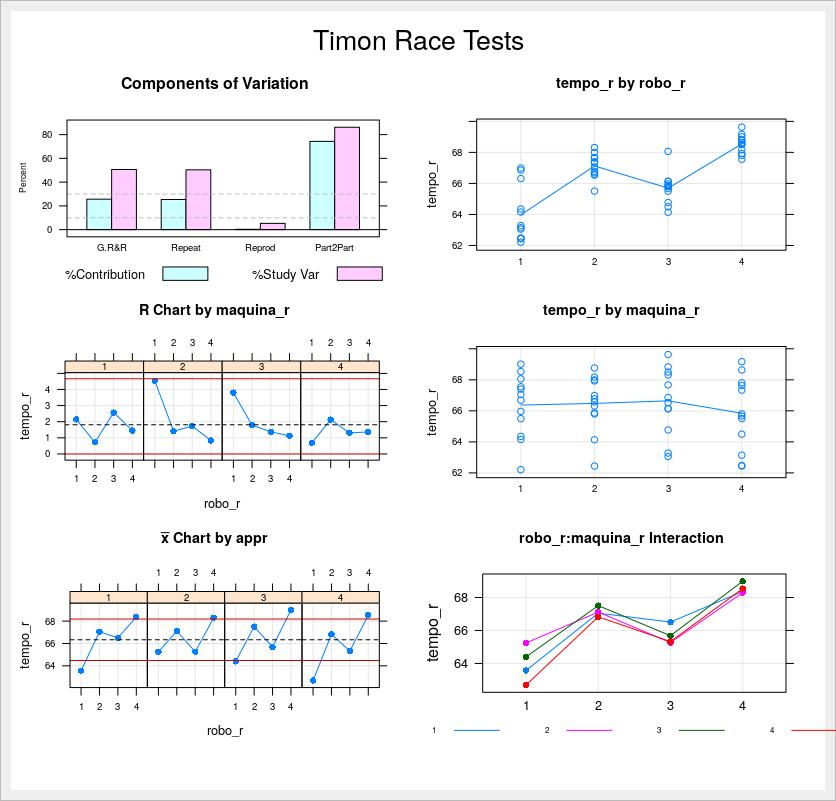
\includegraphics[scale=0.8]{images/timon_race_tests.png}
    \legend{Fonte: Autoria própria.}
\end{figure}

Pode-se observar na (tempo\_r by robo\_r) que robô 4 apresenta um valor de tempo médio maior que os demais, isso ocorre, a priori, devido ao posicionamento do Aruco que sinaliza o fim de percurso da simulação. Também podemos observar em x\_chart by appr que as 4 máquinas apresentarem comportamentos similares na coleta de dados, porém com amplitudes diferentes, o que indica possíveis falhas.

De acordo com a Figura 2, o p valor encontrado é maior que alpha, o que caracteriza uma distribuição normal nos resultados encontrados. Além disso, observa-se um valor de categorias distintas igual a 2 e, como pode ser observado também na Figura 1, maior contribuição vinculada ao item Part-To-Part, elementos considerados positivos para o sistema.
